\documentclass{article}
\usepackage[letter, margin=0.95in]{geometry}
\usepackage{graphicx}
\usepackage{amsmath}

\begin{document}

\title{Explaining Pup Inflation: A Look at @dog\_rates}
\author{Neel Sadafule}
\date{November 29, 2024}
\maketitle

The @dog\_rates Twitter account is famous for rating dogs. But has there been a trend of “pup inflation” over time? Using data from the account, we analyzed whether ratings have grown more generous in recent years.

\section*{The Trend: Is Pup Inflation Real?}
We started by plotting ratings over time and adding a best-fit line. The results revealed a slight upward trend. In our follow-up analysis, we confirmed this statistically: the slope of the trend line was significantly different from zero, proving that @dog\_rates has indeed become more generous. Whether this reflects increasing love for dogs or evolving audience expectations, one thing is clear—dogs are being celebrated more than ever.

\section*{Visualizing the Results}
\subsection*{Scatter Plot with Fit Line}
The scatter plot below shows ratings over time with a clear trendline, demonstrating how ratings have risen.

\begin{center}
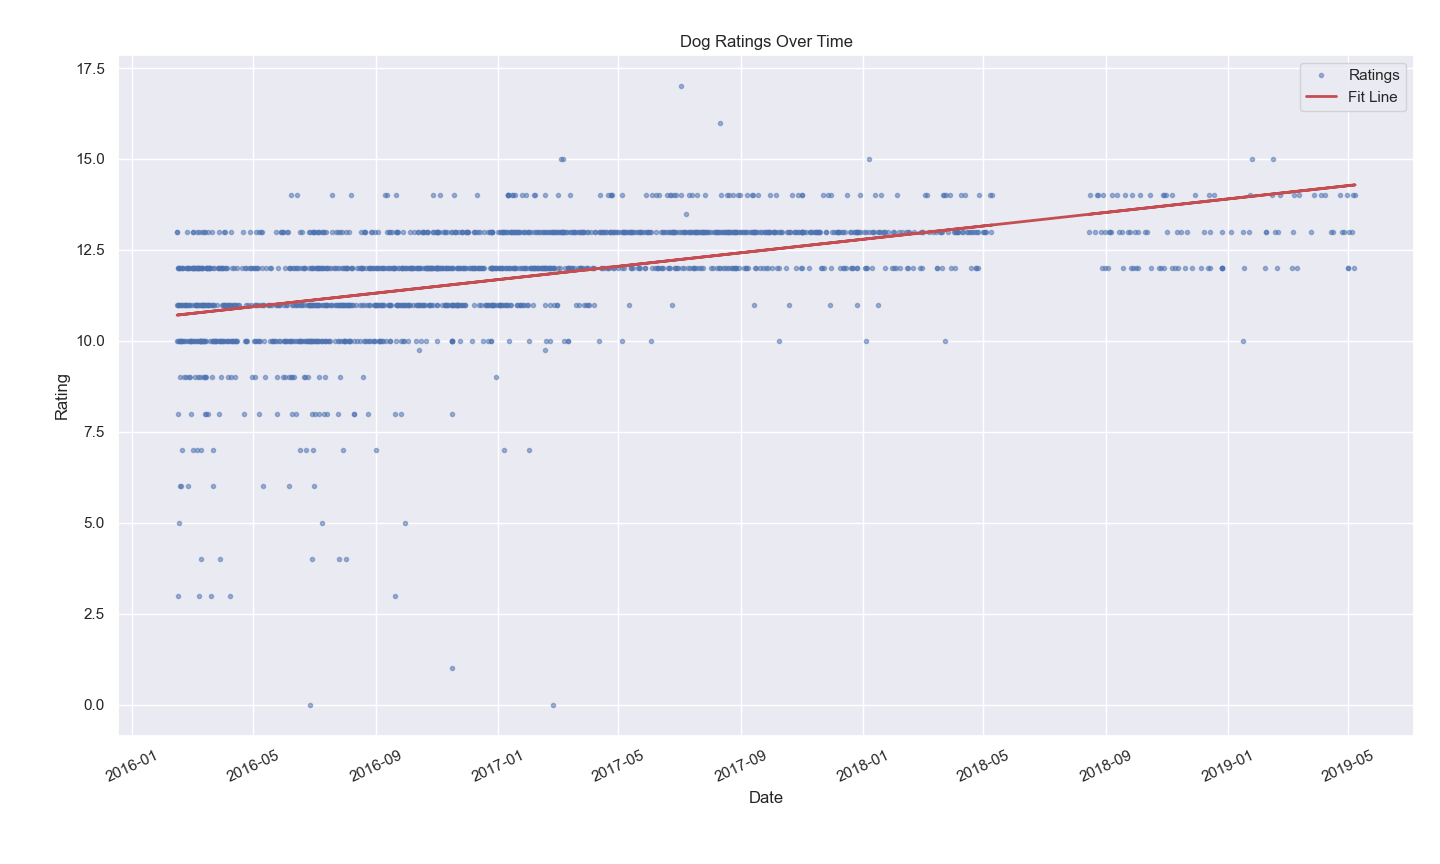
\includegraphics[width=0.8\textwidth]{scatter_plot.png} % Replace with your scatter plot image
\end{center}

\subsection*{Histogram of Residuals}
To evaluate the trend’s accuracy, we plotted the residuals (differences between observed and predicted ratings). These mostly clustered around zero, suggesting the model fits well, with some outliers likely representing truly exceptional pups.

\begin{center}
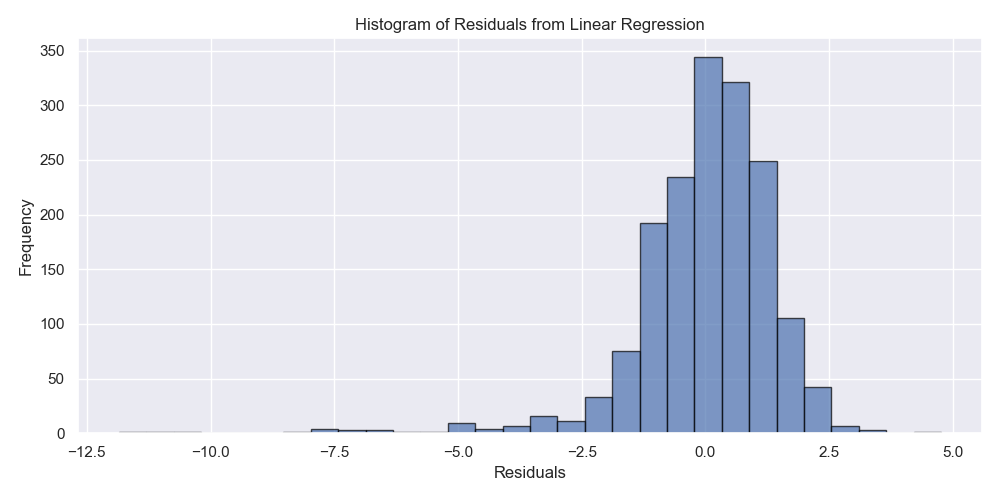
\includegraphics[width=0.8\textwidth]{histogram.png} % Replace with your histogram image
\end{center}

\section*{Conclusion}
In conclusion, pup inflation is real, and it’s a joyful trend. It reminds us that no matter how high the bar is set, dogs will always find a way to leap over it probably while wagging their tails.

\end{document}
